\documentclass{ctexart}
\usepackage{amsmath}
\usepackage{graphicx}
\usepackage{float}
\usepackage{geometry}
\usepackage{hyperref}
\usepackage{tabularx}
\title{动态法测量良导体热导率}
\author{陈启钰\,\,\, 2300011447}
\date{\today}
\begin{document}
	\maketitle
	\newpage
	\section{数据与处理}	
	\subsection{稳定的五组实验曲线}
	稳定的五组曲线(铝管)打印如图\ref{fig:data}所示
	\begin{figure}[h]
		\centering
		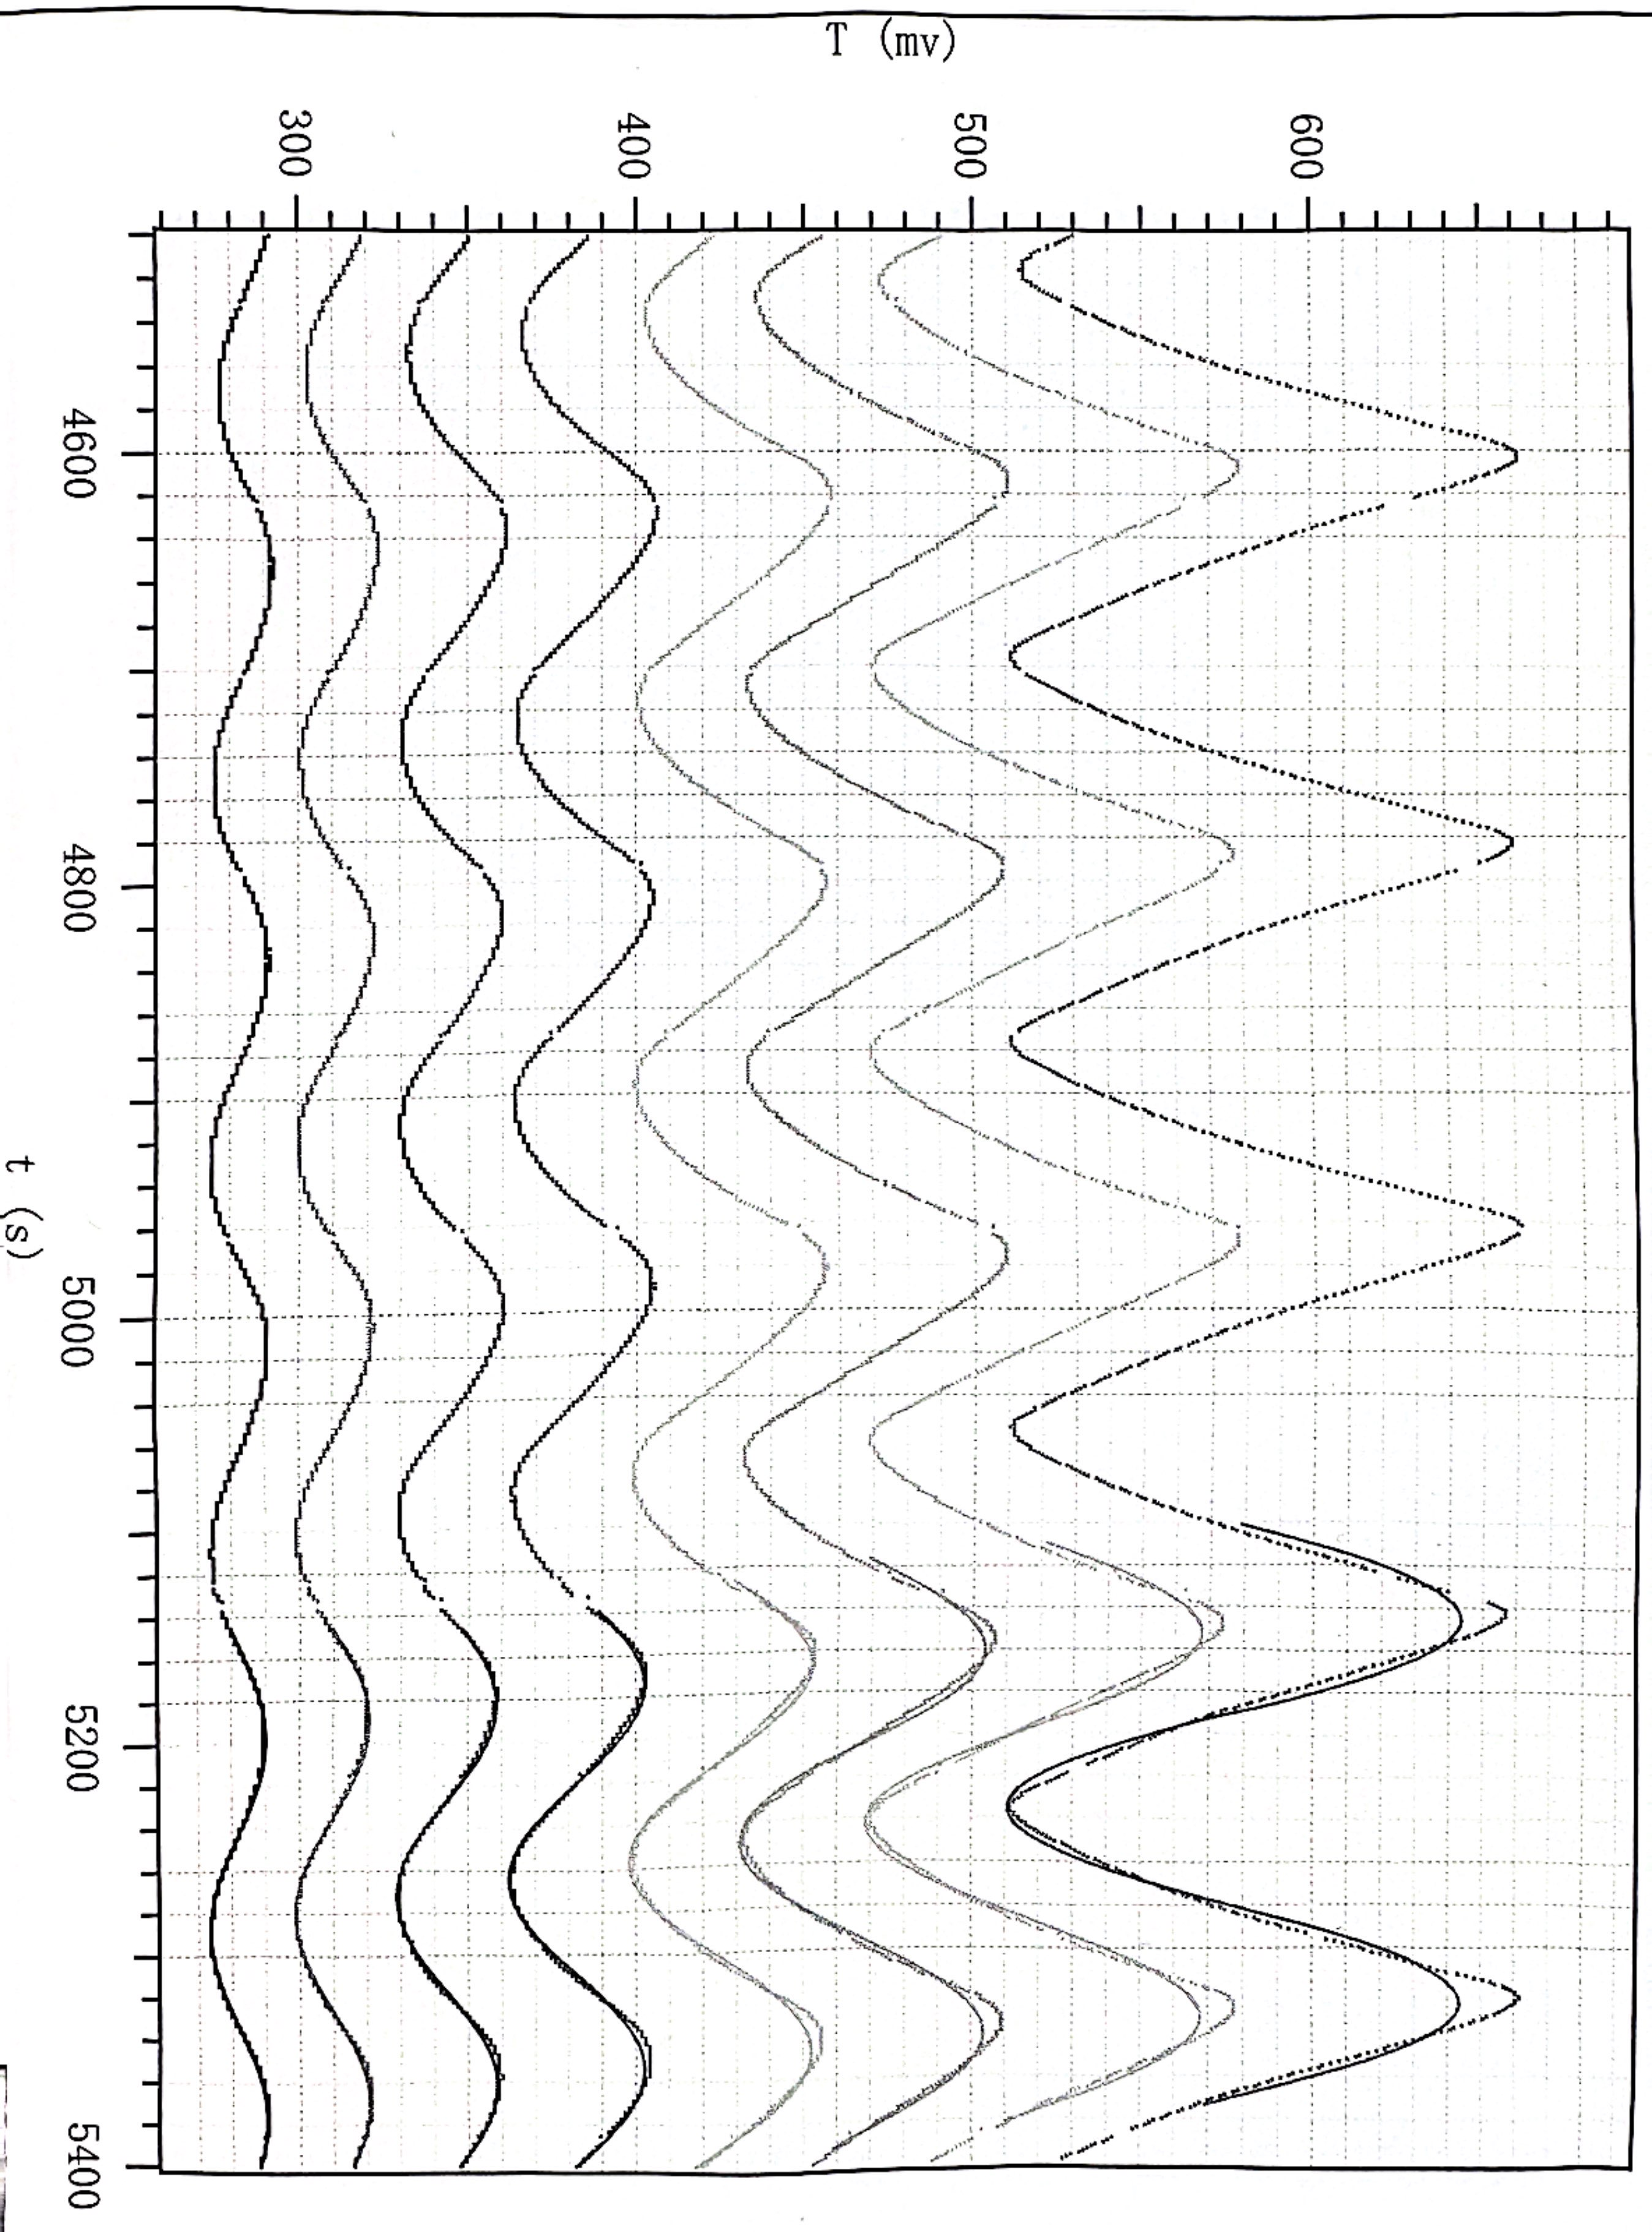
\includegraphics[width=8cm,angle=90]{data.jpg}
		\caption{五组稳定的曲线}
		\label{fig:data}
	\end{figure}
	\subsection{实测数据}
	通过人工读取一组波峰和两组波谷,得到的数据如表\ref{tab:datamanual}所示。实验中水的流量为
	\begin{align}
		v_{\text{cold}}=321\text{mL/min}\\
		v_{\text{hot}}=603\text{mL/min}
	\end{align}
	\begin{table}[H]
		\begin{center}
			\caption{人工测量的数据记录表}
			\begin{tabular}{c|cccccccc}
				$i$&1&2&3&4&5&6&7&8\\
				\hline
				$U_{i\text{波峰}}/\text{mV}$&661.5&577.4&510.8&454.9&444.0&359.8&321.9&292.6\\
				\hline
				$t_{i\text{波峰}}/\text{s}$&5323.54&5329.12&5335.60&5342.77&5350.21&5357.97&5366.39&5373.48\\
				\hline
				$U_{i\text{波谷1}}/\text{mV}$&510.9&496.6&432.6&398.5&361.8&329.5&299.3&273.0\\
				\hline
				$t_{i\text{波谷1}}/\text{s}$&5235.71&5242.06&5249.50&5257.33&5265.06&5272.70&5281.03&5290.63\\
				\hline
				$U_{i\text{波谷2}}/\text{mV}$&510.2&468.9&432.2&399.1&362.4&329.5&298.9&273.4\\
				\hline
				$t_{i\text{波谷2}}/\text{s}$&5415.67&5422.31&5429.55&5437.08&5445.61&5453.14&5463.43&5470.79
				\label{tab:datamanual}
			\end{tabular}
		\end{center}
	\end{table}
	\subsection{热导率的计算}
	\subsubsection{利用人工读取的数据进行计算}
	热波波速可由
	\begin{align}
		v=\frac{il_0}{t_{i+1}-t_1}
	\end{align}
	计算,即有
	\begin{align}
		t_{i+1}-t_1=\frac{il_0}{v}
	\end{align}
	式中$l_0=2\text{cm}$,将$(t_{i+1}-t_1)-i$列表如下
	\begin{table}[H]
		\begin{center}
			\caption{人工测量的数据记录表}
			\begin{tabular}{c|ccccccc}
				$i$&1&2&3&4&5&6&7\\
				\hline
				$t_{i+1}-t_1\text{(波峰)}/\text{s}$&5.58&12.06&19.23&26.67&34.43&42.85&49.94\\
				\hline
				$t_{i+1}-t_1\text{(波谷1)}/\text{s}$&6.35&13.79&19.62&29.35&36.99&45.32&54.92\\
				\hline
				$t_{i+1}-t_1\text{(波谷2)}/\text{s}$&6.64&13.88&21.41&29.94&37.47&47.76&55.12
			\end{tabular}
		\end{center}
	\end{table}
	对波峰进行线性拟合,得到
	\begin{align}
		(t_{i+1}-t_1)_\text{波峰}&=7.495i-2.732\text{s},r=0.9994\\
		(t_{i+1}-t_1)_\text{波谷1}&=8.076i-2.829\text{s},r=0.998\\
		(t_{i+1}-t_1)_\text{波谷2}&=8.188i-2.434\text{s},r=0.9990
	\end{align}
	从而有波速
	\begin{align}
		v_\text{波峰}&=\frac{l_0}{7.495\text{s}}=2.668\times10^{-3}\text{m/s}\\
		v_\text{波谷1}&=2.476\times10^{-3}\text{m/s}\\
		v_\text{波谷2}&=2.443\times10^{-3}\text{m/s}
	\end{align}
	根据热导率计算公式
	\begin{align}
		\kappa=\frac{v^2c\rho}{4\pi}T_\text{period}
	\end{align}
	式中
	\begin{align}
		c=0.897\times10^3\mathrm{J/(K\cdot kg)},\rho=2.70\times10^3\mathrm{kg/m^3},T_\text{period}=180\mathrm{s}
	\end{align}
	计算得到
	\begin{align}
		\kappa_\text{波峰}&=2.46\times 10^2 \mathrm{W/(m\cdot K)}\\
		\kappa_\text{波谷1}&=2.13\times 10^2 \mathrm{W/(m\cdot K)}\\
		\kappa_\text{波谷1}&=2.07\times 10^2 \mathrm{W/(m\cdot K)}
	\end{align}
	\subsubsection{通过正弦拟合得到的数据}
	通过实验室给出的软件对所选的一段波进行正弦拟合,得到的数据列表如下
	\begin{table}[H]
		\begin{center}
			\caption{正弦拟合得到的数据}
			\begin{tabular}{c|cccccccc}
				$i$&1&2&3&4&5&6&7&8\\
				\hline
				$t_{i\text{波峰}}/\text{s}$&4965.7&4972.8&4980.5&4987.4&4995.1&5002.8&5010.9&5018.7\\
				\hline
				$t_{i\text{波谷1}}/\text{s}$&5055.5&5062.5&5070.1&5076.8&5084.5&5092.1&5100.4&5108.2\\
				\hline
				$t_{i\text{波谷2}}/\text{s}$&5235.5&5242.4&5250.1&5256.8&5264.4&5272.2&5280.5&5288.2
			\end{tabular}
		\end{center}
	\end{table}
	软件计算得到的热导率为
	\begin{align}
		\kappa'_\text{波峰}&=2.395\times 10^2 \mathrm{W/(m\cdot K)}\\
		\kappa'_\text{波谷1}&=2.430\times 10^2 \mathrm{W/(m\cdot K)}\\
		\kappa'_\text{波谷2}&=2.421\times 10^2 \mathrm{W/(m\cdot K)}
	\end{align}
	可见,通过软件拟合得到的热导率的值比人工读数然后计算的偏差要更小。
	\subsubsection{通过衰减计算}
	由于有温度$T(x)$的分布
	\begin{align}
		T=T_0-kx+T_\text{m}\exp{\left(-\sqrt{\frac{\omega}{2\alpha}}x\right)}\sin{\left(\omega t-\sqrt{\frac{\omega}{2\alpha}x}\right)}
		\label{eq:sj}
	\end{align}
	忽略$k$,对于相同时间不同位置的峰值或谷值,有
	\begin{align}
		U\propto \exp{\left(-\sqrt{\frac{\omega}{2\alpha}}x\right)}
	\end{align}
	两边取对数,则有
	\begin{align}
		\ln{U}=-\sqrt{\frac{\omega}{2\alpha}}x+\text{C}=-\sqrt{\frac{\pi\rho c}{\kappa T_\text{period}}}x+\text{C}
	\end{align}
	式中$\text{C}$为常数。根据表\ref{tab:datamanual}中的电压值,计算峰峰值,就可以通过衰减规律测量热导率。将$V-x$关系列表如下
	\begin{table}[H]
		\begin{center}
			\caption{衰减法测量热导率的数据}
			\begin{tabular}{c|cccccccc}
				$x/\mathrm{m}$&0.02&0.04&0.06&0.08&0.10&0.12&0.14&0.16\\
				\hline
				$\ln{U}$&5.017&4.550&4.362&4.027&4.405&3.411&3.127&2.965
			\end{tabular}
		\end{center}
	\end{table}
	线性拟合得到
	\begin{align}
		\ln{U}_{\text{波峰}}=-14.26x+5.268,r=0.95
	\end{align}
	计算得到
	\begin{align}
		\kappa''=2.079\times 10^2 \mathrm{W/(m\cdot K)}
	\end{align}
	\section{分析与讨论}
	\subsection{几种方法的比较}
	通过人工测量得到的数据显然要比通过软件进行正弦拟合得到的数据偏差要大,这是因为在人工读数的过程中,鼠标稍微左右移动一点儿,读数就会变化1秒左右(这是因为横轴达到6000秒使得分度值较大)。此外,读数过程中在判断最大值和最小值方面也有一定困难,而且曲线在顶点附近可能是不平滑的。而正弦拟合考虑了整条曲线,拟合得很准确,因此波峰以及波谷的判断是要比人工精准的多。
	
	因此,软件拟合的方法要比人工读数的方法好。
	\subsection{误差分析}
	\subsubsection{系统误差}
	本实验的系统误差来源于样品温度是否达到动态稳定。根据实验中画出来的图\ref{fig:data},可以发现波形并不是完美的正弦波,而是有一定的畸变,而且波形随着时间仍在缓慢变化,说明样品并没有完全达到动态稳定,因此会造成误差。
	\subsubsection{偶然误差}
	偶然误差可能来源于仪器测量几个监测点的温度时,由于温度的涨落或者电压测量本来就带有的偶然性。在人工读数时,选取的波峰、波谷的误差也应该属于偶然误差。
	\newpage
	\section{原始数据}
	\begin{figure}[h]
		\centering
		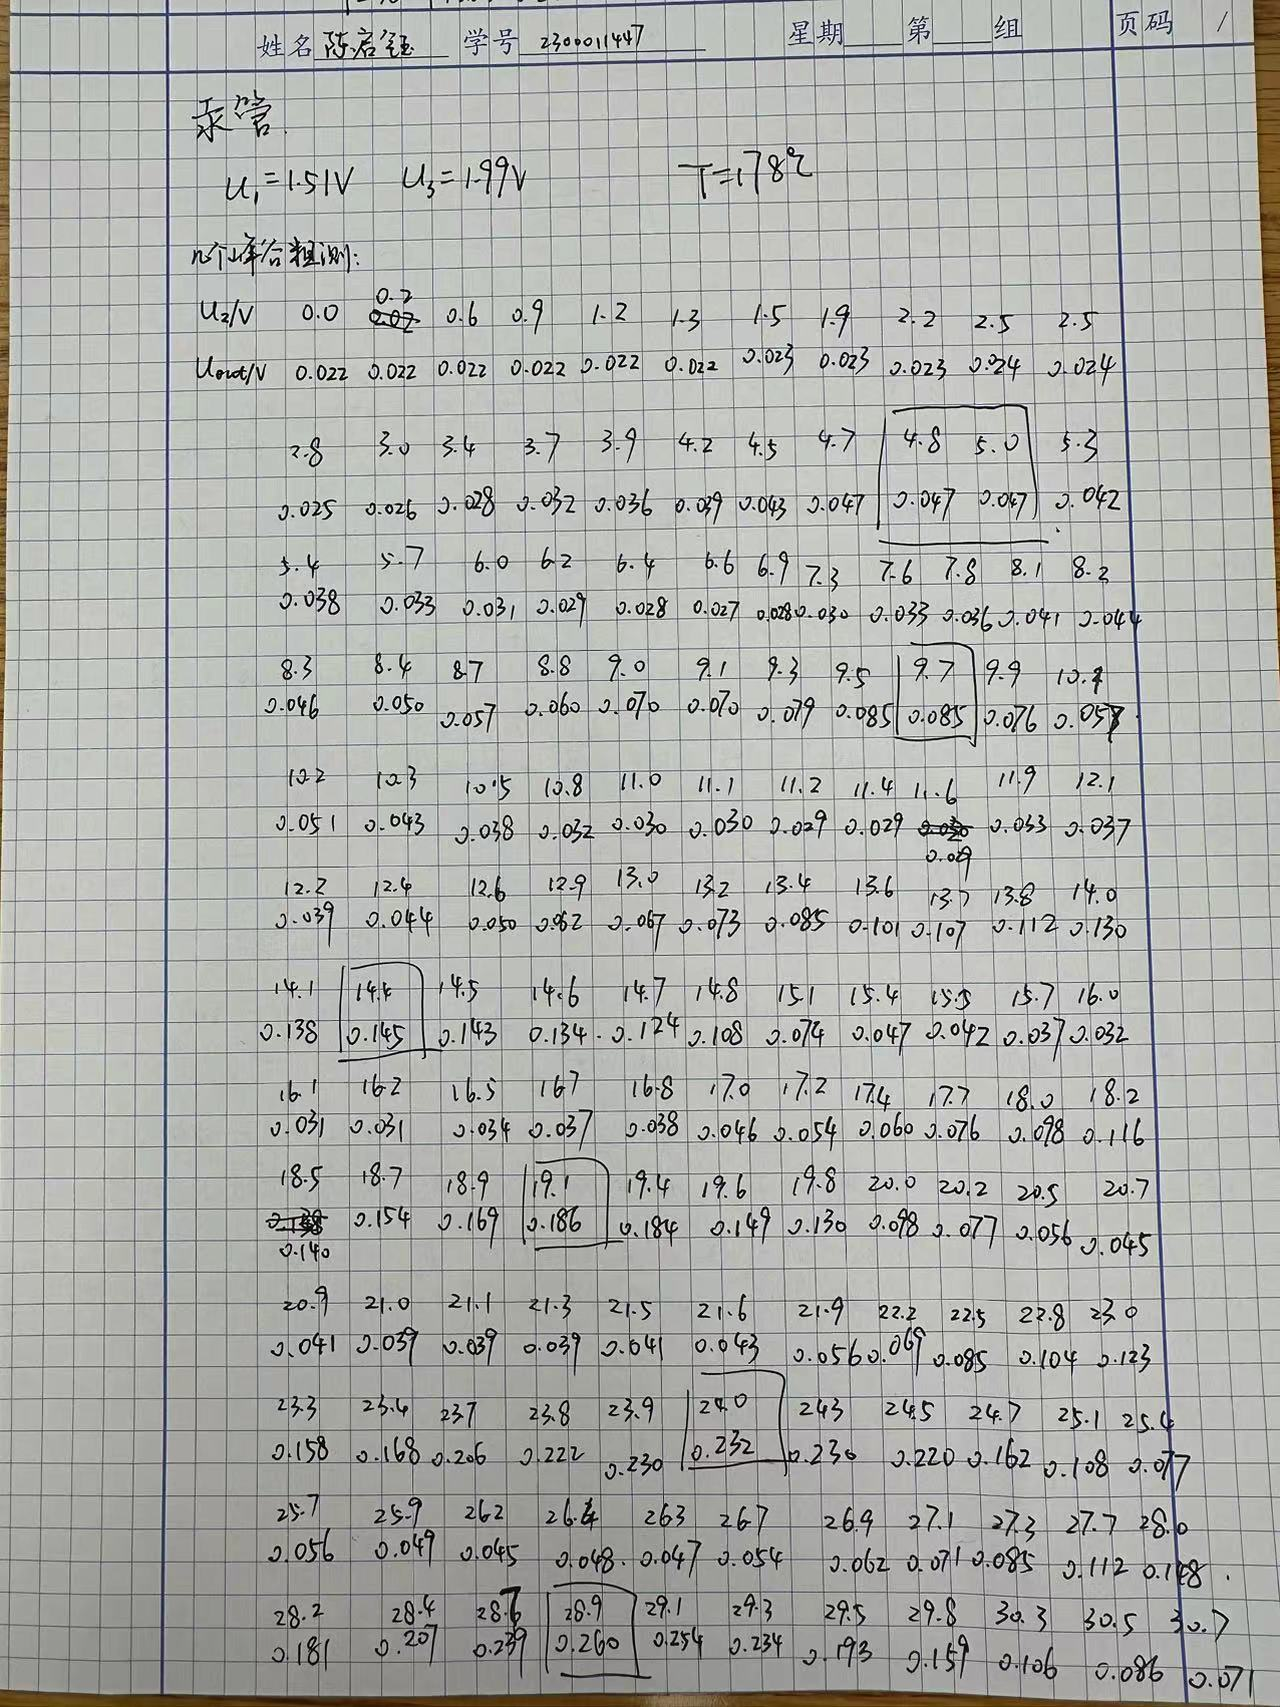
\includegraphics[width=\textwidth,angle=270]{data1.jpg}
	\end{figure}
\end{document}